\mainmatter
\pagestyle{headings}

\chapter{Methodology}
\label{ch:methodology}
\section{Research Questions \& Hypotheses}
To determine the influence of chatbots on the telecom industry, various questions must be asked of the industry's participants. These inquiries are predicated on a hypothesis from which we begin our investigation.\\
\break
Even if reality suggests otherwise, the hypotheses are developed with a favourable expectation in mind.\\
\break
\textbf{Main Question: Do current customer service chatbots know what they are supposed to do?}\\
\break 
Five research questions were formulated to answer this main research question:

\subsubsection{RQ1: Are current customer service chatbots effective in helping people and solving their problems?}
It is illogical to think that there will be people who will keep a good impression of a customer service chatbot after it was unable to help with or solve their existing problem. Multiple studies suggest that it is essential that the execution done by a chatbot is effective \textbf{[WIP: complete studies]}.\\
In a task- oriented chatbot, under which a customer service chatbot can be placed, usefulness is key \citep{brandtzaeg2020}. Solving problems and providing help in an effective and efficient manner is the key to providing a good user experience. It is also crucial that the user's intentions are correctly interpreted and answered adequately.\\
\break
\citep{Verkeyn2018} categorized 28 quality attributes and divided them up in 5 dimensions. Based on these quality attributes, the evaluation of a chatbot is possible (see literature study). Relevant quality attributes that can be linked to the research question serve as the foundation for the hypotheses. In this way, the research question can be reliably tested against reality.\\
\break
\break
Related hypotheses:
\begin{enumerate}
	\item H1: Current customer service chatbots execute requested tasks correctly. Based on \citep{Verkeyn2018} quality attribute “Execute requested tasks” from the dimension “Functionality”
	\item H2: Current customer service chatbots can deliver the same services as a human agent. Based on \citep{Verkeyn2018} quality attribute “Number of services available in the chatbot” from the dimension “Functionality” (reference: \citep{Eeuwen2017})
	\item H3: Current customer service chatbots contain enough knowledge to provide good assistance. Based on \citep{Verkeyn2018} quality attribute “Contains breadth of knowledge” from the dimension “Trustworthiness” (reference: \citep*{Cohen2016, Kuligowska2015})
\end{enumerate}

\subsubsection{RQ2: Are current customer service chatbots easy to use and accessible?}
When a customer service chatbot is effective in helping people, but is so complex or unusable that nobody uses it again, it is rational to assume that this chatbot has not made a good impression. In addition, a chatbot should be easily accessible, so that a high level of service is always present.\\
Here, too, the quality attributes of \citep{Verkeyn2018} serve as the basis for evaluation. Relevant quality attributes that can be linked to the research question serve as the foundation for the hypotheses. In this way, the research question can be reliably tested against reality.\\
\break
\break
Related hypotheses:
\begin{enumerate}
	\item H4: Current customer service chatbots are easy to use. Based on \citep{Verkeyn2018} quality attribute “Ease of use” from the dimension “Efficiency” (reference:\citep*{Candela2018, Duijst2017})
	\item H5: Current customer service chatbots are available at all times (24/7). Based on \citep{Verkeyn2018} quality attribute “Available at all times” from the dimension “Efficiency” (reference: \citep{Wang2019})
\end{enumerate}

\subsubsection{RQ3: Do current customer service chatbots create a pleasant customer experience?}
When a customer uses a service or buys a product from a company, it is important that the customer has a good feeling about how this interaction went. When using a chatbot, a company wants to invoke a good feeling in the user as well. \\
\break
A “pleasant” customer experience can be seen as an experience where the customer is helped in a friendly and smooth way.\\
\break
\break
Related hypotheses:
\begin{enumerate}
	%hypthese 6 gaan we eruit moeten laten, wordt niet ondervraagd in de survey
	\item H6: Current customer service chatbots have a nice user-interface. Based on \citep{Verkeyn2018} quality attribute “User-interface” from the dimension “Graphical appearance” (reference: \citep*{Duijst2017, Kuligowska2015},
	\item H7: Current customer service chatbots create an enjoyable interaction Based on \citep{Verkeyn2018} quality attribute “Create an enjoyable interaction” from the dimension “Humanity” (reference: \citep{Morrissey2013})
\end{enumerate}

\subsubsection{RQ4: Do the business users still prefer to use human over a customer service chatbot?}
Humans have dealt with human interaction for thousands of years. Recently, a new means in the form of a chatbot has come into our lives. It isn’t strange to assume, considering humans are seen as social animals and our history, that a client would still prefer human interaction above interactions with a chatbot. Yet, the literature has a two-sided stance on this matter. Some articles make this statement to be correct \citep{Ashfaq2020} whilst others dispute its facts \citep*{Muizzah2021, Radziwil2021}. Since there is uncertainty, this research might help clear things up.\\
\break
H8: Business users still prefer human interaction above a customer service chatbot.\\
\break
Research hints at many possible problems when interacting with machines which can lead to frustrations. This makes users less likely to want to converse with chatbots. \citep*{Ashfaq2020, brandtzaeg2020, Goot2020} That is why the hypothesis start from the perspective that human-human interaction is still preferred.

\section{Methodology - interviews}
\section{Methodology - survey}
The exact methodology is shown below.\\
\break
The research questions and hypotheses will be investigated by means of a joint survey.\\
\break
These two strategies will be used to generate the most amount of business value possible. For the business, the value is created by comparing the competition and gathering insight into what the customers consider important. For the customer is the value found in better chatbots as a result of the study.\\

\subsection{Are these attributes present for the specific chatbot?}
To find out if the selected attributes are present, several questions will be used to check with the clients using the chatbots. The used questions per research question are listed below.

\subsubsection{RQ1: Are current customer service chatbots effective in helping people and solving their problems?}
\begin{itemize}
	\item H1: Current customer service chatbots execute requested tasks correctly.
	\begin{itemize}
		\item Did the chatbot fulfil your task correctly?
	\end{itemize}
	\item H2: Current customer service chatbots can deliver the same services as a human agent.
	\begin{itemize}
		\item Does the chatbot deliver the same services as a human?
	\end{itemize}
	\item H3: Current customer service chatbots contain enough knowledge to provide good assistance.
	\begin{itemize}
		\item Did the chatbot contain enough knowledge to help with your problem?
	\end{itemize}
\end{itemize}

\subsubsection{RQ2: Are current customer service chatbots easy to use and accessible?}
\begin{itemize}
	\item H4: Current customer service chatbots are easy to use.
	\begin{itemize}
		\item Was the chatbot easy to use?
	\end{itemize}
	\item H5: Current customer service chatbots are available at all times (24/7).
	\begin{itemize}
		\item Is the chatbot available at all times?
	\end{itemize}
\end{itemize}

\subsubsection{RQ3: Do current customer service chatbots create a pleasant customer experience?}
\begin{itemize}
	\item H6: Current customer service chatbots have a nice user-interface.
	\begin{itemize}
		\item Did the chatbot look good?
	\end{itemize}
	\item H7: Current customer service chatbots create an enjoyable interaction.
	\begin{itemize}
		\item Did you enjoy interacting with the chatbot?
	\end{itemize}
\end{itemize}
\ul{Rating scale}\\
For answering the statements, yes/no questions will be used to check the presence of these attributes.\\

\subsubsection{Data Evaluation Method - Comparative Study}
Both providers’ chatbots will be compared to one another to see which attributes are present in which chatbot.\\

\subsection{How important are these attributes for the clients?}
The research questions and hypotheses will be investigated/evaluated by means of the proven KANO method. The method of application is inspired by the study of \citep{Verkeyn2018}.\\
\break
To find out which of the chose 7 attributes types are seen as important, the following questions per category will be used.

\subsubsection{Under ``Effective in helping people and solving their problems"}
\begin{enumerate}
	\item Execute requested tasks
	\begin{itemize}
		\item The chatbot (DOES NOT) execute(s) every/any requested task that can reasonably be expected to be executed successfully.
	\end{itemize}
	\item Number of services available in the chatbot
	\begin{itemize}
		\item The chatbot can (NOT) perform the same services as a human agent.
	\end{itemize}
	\item Contains breadth of knowledge
	\begin{itemize}
		\item The chatbot knows at least as much as an expert in the same industry/service./ The chatbot knows less than an expert in the same industry/service.
	\end{itemize}
\end{enumerate}

\subsubsection{Under "Ease of use and accessibility"}
\begin{enumerate}
	\item Ease of use
	\begin{itemize}
		\item The chatbot is (NOT) self-explanatory in its use.
	\end{itemize}
	\item Available at all times
	\begin{itemize}
		\item The chatbot is (NOT) available at all times.
	\end{itemize}
\end{enumerate}

\subsubsection{Under "Pleasant customer experience"}
\begin{enumerate}
	\item User-interface
	\begin{itemize}
		\item The chatbot user-interface has/does NOT have a good-looking lay-out.
	\end{itemize}
	\item Create an enjoyable interaction
	\begin{itemize}
		\item The chatbot (DOES NOT) communicate(s) in a robotic, non-empathic way./ The chatbot interacts in an enjoyable way.
	\end{itemize}
\end{enumerate}
\ul{Rating scale}\\
For answering the statements, a five-level rating scale in the spirit of the one drawn up by \citep{KANO1984}, will be used.\\
\break
The levels are as follows:\\
\begin{enumerate}
	\item I dislike it
	\item I can live with it
	\item I am neutral
	\item I expect it
	\item I like it
\end{enumerate}
This scale allows users to express how much they agree with a given statement.\\

\subsubsection{Data Evaluation Method - Comparative Study}
To be able to answer the second main question, there is a need for an evaluation method that will list the general user importance for each quality attribute. Kano is a tool that can satisfy these desires. The Kano Model gives more insight into the fact that the performance of the quality attributes is not in a linear relationship with the corresponding customer satisfaction \citep{KANO1984}. Kano offers the possibility to divide the quality attributes into five categories that each have different effects on customer satisfaction (Performance, Must-Be, Attractive, Reverse, Indifferent). This division is done on the basis of the answers obtained from the survey (questions with five-level rating scale).\\

\begin{figure}[ht]
	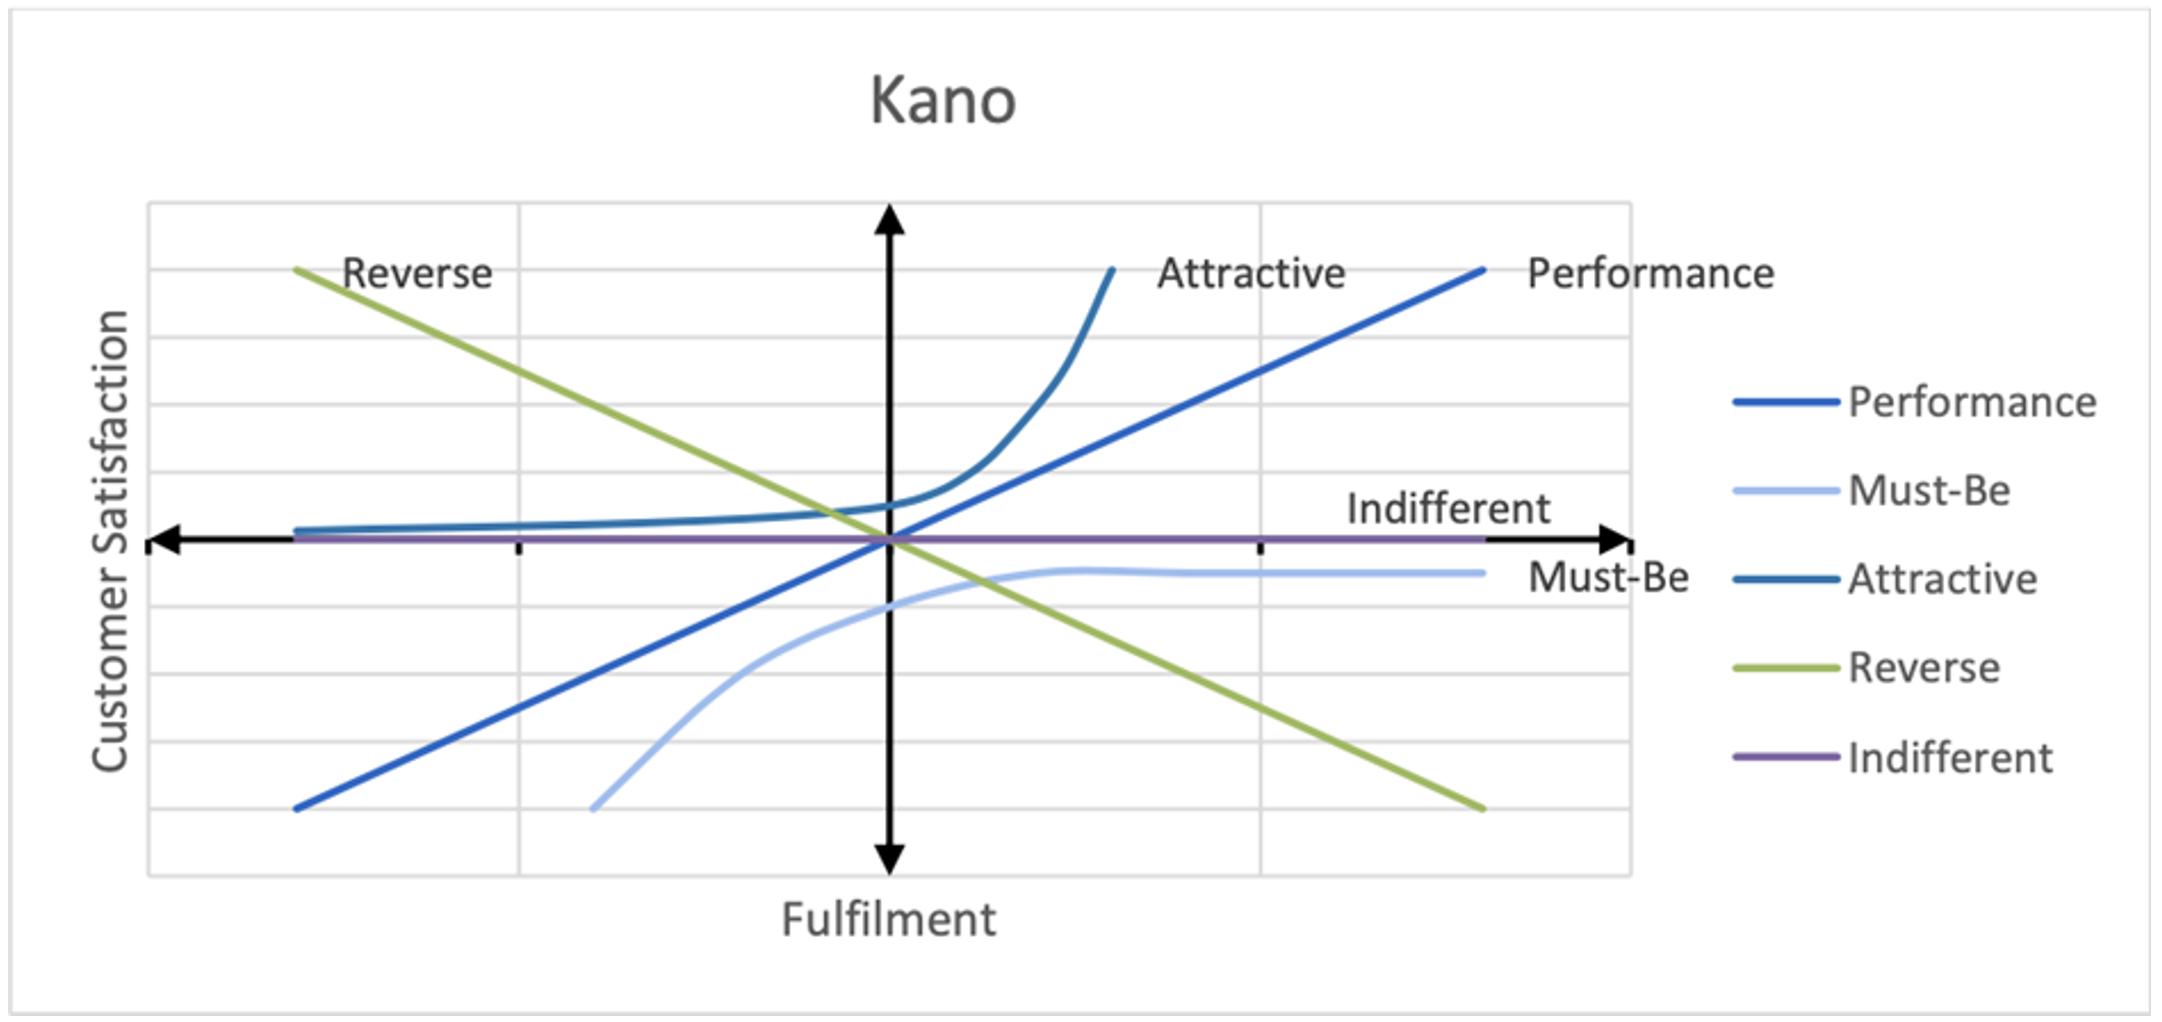
\includegraphics[scale=0.35]{../LaTeX/Figures/KANO.png}
	\caption{Five categories of quality attributes \citep{KANO1984}.}
	\label{fig:kano}
\end{figure}
\break
The five categories can be represented visually as in Figure \ref{fig:kano}, each category showing a different relationship.\\
\break
Attractive: if a quality attribute from this category is more present, the customer satisfaction will increase more than linearly. When the quality attribute is not present, the customer will have neither a positive nor negative customer satisfaction.\\
\break
Performance: When a quality attribute from this category is present, the customer satisfaction will increase linearly. If the quality attribute is not present, then this will result in a negative customer satisfaction.\\
\break
Indifferent: If a quality attribute from this category is present, then this has no effect on customer satisfaction.\\
\break
Must-Be: The customer considers this kind of quality attribute as necessary, when it is not present, the customer satisfaction will be drastically low.\\
\break
Reverse: The more these quality attributes are present, the worse the customer satisfaction. The customer satisfaction increases when they are less present.\\

\subsection{Survey arrangement}
This survey is divided up into 4 parts, following the 4 research questions.\\
\break
\ul{Part 1 - Are current customer service chatbots effective in helping people and solving their problems?}\\
In this part, questions are asked about the effective processing of tasks and knowledge.\\
\break
\ul{Part 2 - Are current customer service chatbots easy to use and accessible?}\\
This part asks questions about ease of use and the availability of customer service chatbots.\\
\break
\ul{Part 3 - Do current customer service chatbots create a pleasant customer experience?}\\
In this part, questions are asked about customer experience.\\
\break
\ul{Part 4 - Do the consumer still prefer to use human over a Chatbot?}\\
In this part, the respondent is asked if he/she prefers a chatbot or a human agent.\\ 

\subsection{Target group}
The target group of the study will not be filtered on age or any other demographic aspects, rather we will focus on the telecom sector. Both the providers of the teleservices and the clients using these services will be targeted.

% Changed files:
% - Methodologie.tex
% - ref.tex
% - LiteratureStudy.tex